\newpage
\subsection{token}
\label{ss:token}
Das package \emph{token} (siehe Abbildung \ref{fig:tokenPackage}) vereint s"amtliche Klassen, die ben"otigt werden um einen Domino erstellen zu k"onnen. 

\begin{figure}
	\centering
	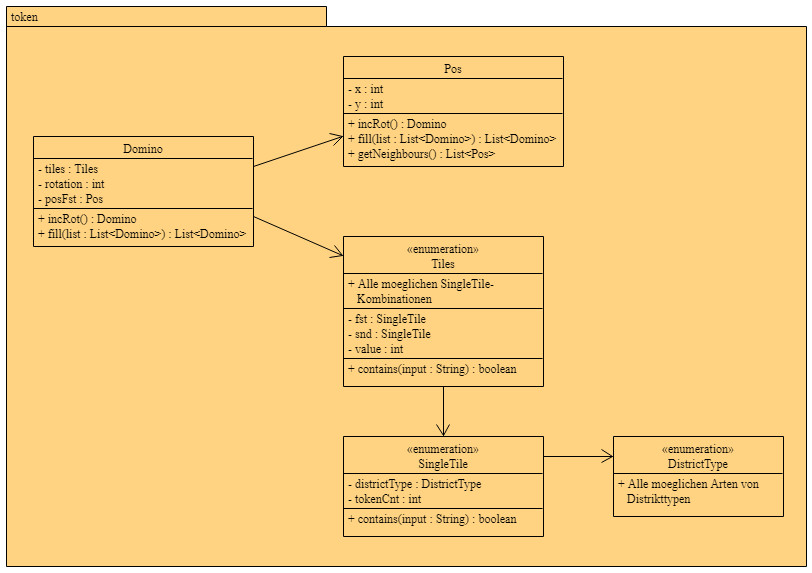
\includegraphics{pics/tokenPackage}
	\caption{UML-Darstellung des token packages}
	\label{fig:tokenPackage}
\end{figure}

\paragraph{Pos}
\label{par:pos}
Diese Klasse wurde von der Bonusaufgabe der PS2-"Ubungung "ubernommen. Es wurde lediglich die \emph{toString()}-Methode sowie \emph{getNeighbours()} abge"andert und einige Konstanten hinzugef"ugt um den Checkstyle-Richtilinien 
(siehe Abschnitt \ref{sec:entwicklungskonfiguration} - \nameref{sec:entwicklungskonfiguration}) 
folge zu leisten. Dennoch folgt hier ein kurzer "Uberblick "uber diese Klasse: 

Eine Position setzt sich aus einer X- und einer Y-Komponente zusammen. Diese sind als \emph{final} deklariert und k"onnen somit nicht ver"andert werden. Neben dem Konstruktor und diversen Gettern gibt es eine Methode um festzustellen ob sich eine gegebene Position neben der Position des Objekts befindet. Dazu wird ein die Differenz der beiden jeweils gleichnamigen Komponenten gebildet und am Ende verglichen, ob nur jeweils eine der beiden Differenzen gleich Null ist (siehe Listing \ref{lst:pos_isNextTo}). 

\begin{lstlisting}[float,style=CodeHighlighting,caption=Pos - isNextTo(),label=lst:pos_isNextTo]
public boolean isNextTo(Pos p) {
    int xDiff = Math.abs(x - p.x());
	int yDiff = Math.abs(y - p.y());
	return (xDiff == 1 && yDiff == 0
            || xDiff == 0 && yDiff == 1);
}
\end{lstlisting}

Die Methode \emph{getNeighbours()} liefert eine Arraylist der vier Nachbarn. Hierzu wird eine Liste initialisiert und mit neuen Positionen bef"ullt, deren X- und Y-Komponenten entsprechend modifiziert werden (siehe Listing \ref{lst:pos_getNeighbours}). 

\begin{lstlisting}[float,style=CodeHighlighting,caption=Pos - getNeighbours(),label=lst:pos_getNeighbours]
public List<Pos> getNeighbours() {
    List<Pos> neighbours = new ArrayList<>();
    neighbours.add(LEFT_ROT, new Pos(this.x - 1, this.y));
    neighbours.add(DOWN_ROT, new Pos(this.x, this.y - 1));
    neighbours.add(RIGHT_ROT, new Pos(this.x + 1, this.y));
    neighbours.add(UP_ROT, new Pos(this.x, this.y + 1));
    return neighbours;
}
\end{lstlisting}

Eine \emph{equals}-Methode wurde ebenfalls implementiert, diese vergleicht allerdings nur die jeweiligen x- und y-Komponenten der beiden Positionen. Bei der \emph{toString}-Methode werden die beiden Komponenten, zwischen einem Klammernpaar und mit Komma getrennt, ausgegeben. 

\paragraph{DistrictType}
\label{par:districtType}
In diesem Aufz"ahlungstyp werden die m"oglichen Kategorien der Distrikte aufgef"uhrt. Wichtig hierbei, auch ein leeres Feld sowie das Stadtzentrum besitzen einen Typ (siehe listing \ref{lst:districtType}). 
Dieser Aufz"ahlungstyp spielt vor allem beim Ausz"ahlen der Punkte bzw. dem Verwalten der verschiedenen Distrikte eine wichtige Rolle. 
\begin{lstlisting}[float,style=CodeHighlighting,caption=DistrictType,label=lst:districtType]
public enum DistrictType {
    EMPTY_CELL, CENTER, AMUSEMENT, INDUSTRY, OFFICE, PARK, SHOPPING, HOME
}
\end{lstlisting}

\paragraph{SingleTile}
\label{par:singleTile}
Dieser Aufz"ahlungstyp repr"asentiert einen Domino Aufdruck. 

Ein Konstruktur verbindet die Enum-Darstellung mit einem Distrikttypen und einer Anzahl an Punkten, welche auf dem betrachteten Tile verf"ugbar sind (siehe Listing \ref{lst:singleTile}).

Au"serdem verf"ugt der Aufz"ahlungstyp "uber Getter f"ur beide Felder und eine Methode, die "uberpr"uft, ob eine gegebene String-Repr"asentation dem Wert eines der Enumobjekte entspricht. Hierzu wird eine Schleife durchlaufen, die beim Fund mit \emph{true} und ansonsten mit \emph{false} abbricht. 

\begin{lstlisting}[style=CodeHighlighting,float,caption=singleTile,label=lst:singleTile]
CC(CENTER, 0), EC(EMPTY_CELL, 0),
A0(AMUSEMENT, 0), A1(AMUSEMENT, 1), A2(AMUSEMENT, 2), A3(AMUSEMENT, 3),
I0(INDUSTRY, 0), I1(INDUSTRY, 1), I2(INDUSTRY, 2), I3(INDUSTRY, 3),
O0(OFFICE, 0), O1(OFFICE, 1), O2(OFFICE, 2), O3(OFFICE, 3),
P0(PARK, 0), P1(PARK, 1), P2(PARK, 2), P3(PARK, 3),
S0(SHOPPING, 0), S1(SHOPPING, 1), S2(SHOPPING, 2), S3(SHOPPING, 3),
H0(HOME, 0), H1(HOME, 1), H2(HOME, 2), H3(HOME, 3);

private DistrictType districtType;

private int tokenCnt;

SingleTile(DistrictType disctrictType, int tokenCnt) {
    this.districtType = disctrictType;
    this.tokenCnt = tokenCnt;
}
\end{lstlisting}

\begin{lstlisting}[style=CodeHighlighting,float,caption=Tiles,label=lst:tiles]
P0P0_Val1(P0, P0, 1),
P0P0_Val2(P0, P0, 2),
...
O0I2_Val47(O0, I2, 47),
P0I3_Val48(P0, I3, 48);

public static final int TILES_CNT = Tiles.values().length;

private final SingleTile fst;
private final SingleTile snd;

private final int value;

Tiles(SingleTile fst, SingleTile snd, int value) {
    this.fst = fst;
    this.snd = snd;
    this.value = value;
}
\end{lstlisting}

\clearpage
\paragraph{Tiles}
\label{par:tiles}
Dieser Aufz"ahlungstyp beschreibt alle m"oglichen \emph{SingleTile}-Kombinationen, die im Stapel einer normalen Partie des Spiels m"oglich sind (siehe listing \ref{lst:tiles}). 

Auch hier gibt es wieder einen Konstruktor, der diverse Werte an die jeweiligen Enum-Werte bindet. Es werden neben den beiden SingleTile-Kombinationen auch der Wert dieser spezifischen Kombination gespeichert. Der Wert dient dem Sortieren der B"anke und wurde aus der Aufgabenstellung entnommen (wurde also nicht willk"urlich festgelegt). 

Um von au"serhalb einfacher bestimmte Tile-Kombinationen zu erstellen und das Testen einfacher gestalten zu k"onnen, wurden mehrere Methoden eingef"uhrt die dies erleichtern sollen. Diese sind allerdings im Hauptprogramm nicht von Bedeutung. Neben sonstigen Gettern besitzt diese Klasse lediglich eine \emph{toString()}-Methode, wo nur die ersten 4 Buchstaben der Enum-Werte zur"uckgegeben werden, da diese die Tile-Kombination angeben. Der Wert der Kombination entf"allt hierbei (ist aber in dieser Methode auch unbedeutend).

\paragraph{Domino}
\label{par:domino}
Diese Klasse vereint s"amtliche zuvor genannten Datenstrukturen. 

Ein Domino besitzt eine bestimmte Kombination aus SingleTiles und einer Rotation sowie Position. Letztere beiden beziehen sich auf ein Board, nicht auf eine Bank oder dergleichen. Um eine gegebene Liste zu f"ullen wird die Methode \emph{fill} bereitgestellt. Hierbei wird eine gegebene Liste geleert und mit allen m"oglichen unterschiedlichen Dominos gef"ullt (siehe listing \ref{lst:domino_fill}, \nameref{lst:domino_fill}). Um einen Domino auf einem Spielfeld zu platzieren muss es m"oglich sein seine Position sowie Rotation zu ver"andern, dies geschieht "uber die Methoden \emph{setPosition()} und \emph{incRot() / setRotation()}. \emph{incRot()} inkrementiert hierbei die Rotation um neunzig Grad. Au"serdem ist diese Klasse in der Lage mittels der \emph{toFile()}-Methode einen Zeichenfolge zu generieren um die Tile-Kombination des Steins sp"ater abspeichern zu k"onnen. Hierbei wird allerdings die \emph{toString()}-Methode der Tile-Kombination aufgerufen. Als Letztes implementiert die Domino Klasse noch das Interface \emph{Comparable} um sp"ater Dominos per \emph{Collections.sort(...)} einfacher Sortieren zu k"onnen. Hierbei wird jeweils auf den Wert der Tile-Kombination geschaut (siehe \ref{lst:domino_compareTo}, \nameref{lst:domino_compareTo}). 

\begin{lstlisting}[float,style=CodeHighlighting,caption=Domino - fill,label=lst:domino_fill]
public static List<Domino> fill(List<Domino> list) {
    if (null == list) {
        list = new LinkedList<>();
    } else {
        list.clear();
    }
    for (Tiles tile : Tiles.values()) {
        list.add(new Domino(tile, DEFAULT_POS));
    }
    return list;
}
\end{lstlisting}

\begin{lstlisting}[style=CodeHighlighting,caption=Domino - compareTo,label=lst:domino_compareTo]
@Override
public int compareTo(Object o) {
    assert null != o && (o instanceof Domino);
    Domino other = (Domino) o;
    return this.tiles.getValue() - other.tiles.getValue();
}
\end{lstlisting}